\documentclass{standalone}
\usepackage{tikz}

\begin{document}
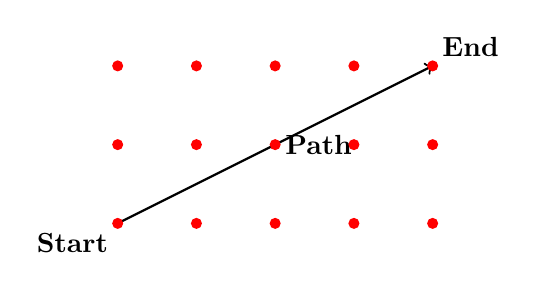
\begin{tikzpicture}[scale=1]
    % Define the coordinates
    \def\ga{4}
    \def\gb{2}
    \def\g{4} % g+1=5 implies g=4

    % Calculate the coordinates
    \pgfmathsetmacro{\xstart}{0}
    \pgfmathsetmacro{\ystart}{0}
    \pgfmathsetmacro{\xend}{\ga}
    \pgfmathsetmacro{\yend}{\gb}

    % Draw the path
    \draw[thick,->] (\xstart,\ystart) -- node[midway,right] {$\textbf{Path}$} (\xend,\yend);

    % Mark the lattice points
    \foreach \i in {0,...,\g} {
        \foreach \j in {0,...,\gb} {
            \fill[red] (\i,\j) circle (2pt);
        }
    }

    % Label the starting and ending points
    \node[below left] at (\xstart,\ystart) {\textbf{Start}};
    \node[above right] at (\xend,\yend) {\textbf{End}};
\end{tikzpicture}
\end{document}